\subsection{Reusable and Consumable Resources}

A reusable resource is used by only one process at a time and is not depleted by that use.
Reusable resources include processors, I/O channels, main and secondary memory, devices, and data structures such as files, databases and semaphores.
Processes obtain reusable resources and later release them for use by other processes.
A deadlock may occur if each process holds one such resource and requests another.

A consumable resource is created (or produced) and later destroyed (or consumed).
Consumable resources include interrupts, signals, messages and information in I/O buffers.
A deadlock may occur if two processes request information from each other at the same time.
Neither can send the required information because both are waiting for a response.

\subsection{Deadlock Conditions}

A deadlock is a permanent blocking of a set of processes competing for resources.
It is a circular resource conflict between a set of processes that occurs when each process currently holds a resource requested by another process and, therefore, each process is also waiting for another process to release its resource.

There exist four conditions that lead to a deadlock.
The first three are preconditions that, when all hold true, may lead to a deadlock.
If the forth condition occurs in addition to the first three, it is inevitable that a deadlock shall occur.

\begin{enumerate}
  \item Mutual exclusion --- only one process may use a resource at a time
  \item Hold-and-wait --- a process can hold a resource while it is waiting for other resources to become available
  \item No preemption --- processes cannot be interrupted to free their resources by force
  \item Circular wait --- processes wait for each other to release resources they wish to acquire, leading to a closed chain of processes
\end{enumerate}

A deadlock occurs when a circular wait occurs and cannot be resolved.
A circular wait cannot be resolved if the three preconditions are true.
Thus, if the first three conditions occur, there is a possibility of a deadlock, and if all four conditions occur there is an inevitable deadlock.

\subsection{Resource Allocation Graphs}

A resource allocation graph is a directed graph that depicts the state of a system of resources and processes.

\begin{figure}[htp]
  \centering
  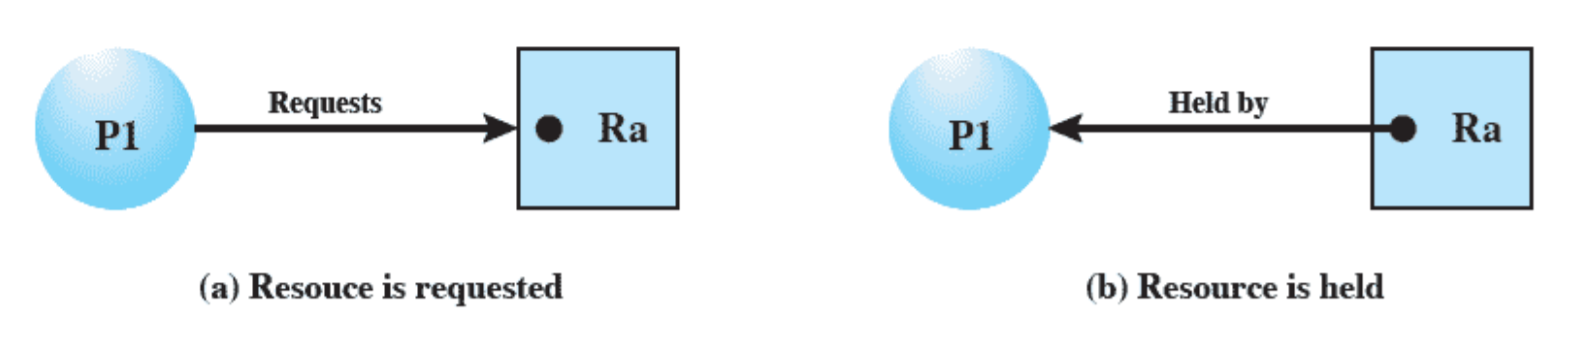
\includegraphics[width=15cm]{unit-15/figures/resource-graph-1.png}
  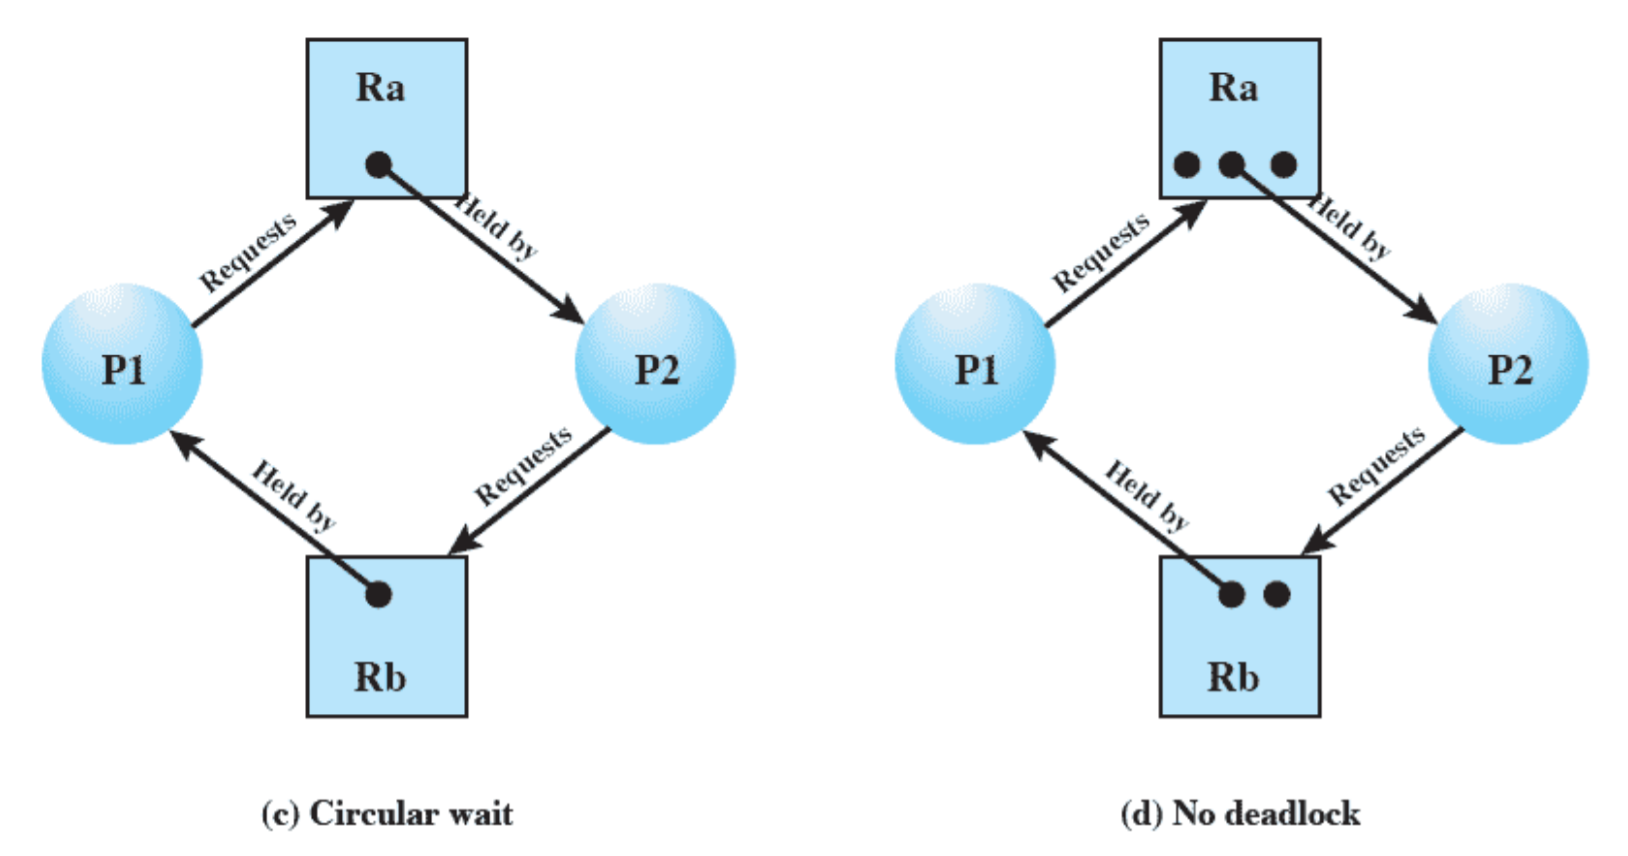
\includegraphics[width=15cm]{unit-15/figures/resource-graph-2.png}
\end{figure}

\subsection{Deadlock Handling}

Deadlocks can be handled through three methods.

\begin{itemize}
  \item Deadlock prevention
  \begin{itemize}
    \item Avoid at least one of the four deadlock conditions
  \end{itemize}
  \item Deadlock avoidance
  \begin{itemize}
    \item Requests for resources whose reservation may lead to deadlock are not granted
  \end{itemize}
  \item Deadlock detection and recovery
  \begin{itemize}
    \item No restriction on resource allocation
    \item Periodic check for deadlocks
    \item When a deadlock is detected, recovery mechanisms are employed
  \end{itemize}
\end{itemize}

\subsection{Deadlock Prevention}

In a deadlock prevention system, the OS is designed to prevent deadlocks from occurring.
The avoidance of the three preconditions is known as `indirect deadlock prevention'.
The avoidance of the final condition is known as `direct deadlock prevention'.

\subsubsection{Mutual Exclusion Prevention}

The mutual exclusion precondition cannot be avoided, as a lack of mutual exclusion may lead to race conditions.

\subsubsection{Hold-and-Wait Prevention}

The hold-and-wait precondition may be avoided by preallocating all required resources in advance and blocking a process until all its resources become available.
This results in long delays for processes, as well as low concurrency and inefficient utilisation of resources.
It is also difficult to achieve since a process may not know in advance what resources it may require.

\subsubsection{No Preemption Prevention}

The avoidance of this condition may be achieved in different ways.
If a process is holding a resource and is denied a request for another resource, it may be preempted.
Alternatively, the process holding the other resource may be preempted.
These methods are only possible if the state of the resources can be saved and restored so that the preempted process may resume execution.

\subsubsection{Circular Wait Prevention}

One method of direct deadlock prevention is to associate an index to each resource.
A process that requires multiple resources must acquire them in ascending index order.
For example, if two processes are competing for resource~1 and resource~2, the first process will acquire resource~1 and is free to acquire resource~2, since the second process cannot acquire either; the second process cannot acquire resource~2 before resource~1, and cannot access resource~1 because it is locked.
This method of resource ordering to prevent circular waits is usually inefficient because processes that use common resources are forced to execute in series rather than parallel.

\subsection{Deadlock Avoidance}

In a deadlock avoidance system, the decision of whether to grant a resource allocation is made dynamically depending on whether it is at all possible that such a request may lead to a deadlock.
This method requires knowledge of future resource requests.
The three preconditions are not avoided.
Instead, intelligent decisions are made when allocating resources.

\begin{itemize}
  \item Process initiation denial --- do not start a process if its demands may lead to deadlock
  \item Resource allocation denial --- do not grant an incremental resource request to a process if the allocation may lead to deadlock
\end{itemize}

\subsubsection{The Resource Matrix System}

Resources and process that require them can be represented using vectors and matrices.
The system resource vector \( \mathbf{r} \) is a vector of the total number of instances of each resource in the system.

\begin{equation*}
  \mathbf{r} = \left[ r_1, r_2, \ldots, r_n \right]
\end{equation*}

The available resource vector \( \mathbf{v} \) is a vector of all available resources (resources that are not in use).

\begin{equation*}
  \mathbf{v} = \left[ v_1, v_2, \ldots, v_n \right]
\end{equation*}

The claim matrix \( \mathbf{C} \) represents the resource requirement of each process.
An element \( c_{pr} \) is the number of instances of resource \( r \) required by process \( p \).
Each row \( \mathbf{c}_p \) represents the total resource claim of process \( p \).

\begin{equation*}
  \mathbf{C} = \begin{bmatrix}
    c_{11} & c_{12} & \ldots & c_{1n} \\
    c_{21} & c_{22} & \ldots & c_{2n} \\
    \vdots & \vdots & \ddots & \vdots \\
    c_{m1} & c_{m2} & \ldots & c_{mn} \\
  \end{bmatrix}
\end{equation*}

The allocation matrix \( \mathbf{A} \) represents the resource allocation of each process.
An element \( a_{pr} \) is the number of instances of resource \( r \) allocated to process \( p \).
Each row \( \mathbf{a}_p \) represents the total resource allocation of process \( p \).

\begin{equation*}
  \mathbf{A} = \begin{bmatrix}
    a_{11} & a_{12} & \ldots & a_{1n} \\
    a_{21} & a_{22} & \ldots & a_{2n} \\
    \vdots & \vdots & \ddots & \vdots \\
    a_{m1} & a_{m2} & \ldots & a_{mn} \\
  \end{bmatrix}
\end{equation*}

All the resources in the system are either available or allocated.

\begin{equation*}
  r_r = v_r + \sum_p a_{pr} \quad \forall r
\end{equation*}

No process may claim more instances of a resource than exist in the system.

\begin{equation*}
  c_{pr} \le r_r \quad \forall p, r
\end{equation*}

No process is allocated more instances of a resource than it claims.

\begin{equation*}
  a_{pr} \le c_{pr} \quad \forall p, r
\end{equation*}

\subsubsection{Process Initiation Denial}

A new process \( \left( n + 1 \right) \) is initiated only if the sum of claims of the new process and all the currently running processes can be met by the system.

\begin{equation*}
  r_r \ge c_{\left( n + 1 \right) r} + \sum_{p = 1}^n c_{pr} \quad \forall r
\end{equation*}

This deadlock avoidance scheme assumes the worst possible scenario --- that all processes will demand their resources at the same time.

\subsubsection{Resource Allocation Denial}

Resource allocation denial is achieved through the `banker's algorithm'.
A process is only allocated a resource if the system will remain in a safe state --- a state in which there exists at least one sequence of resource allocations that does not result in a deadlock.

A system is in a safe state if any of the participating processes can run to completion with the resources available, i.e.\ the difference between the requirement and allocation of any process can be met with the resources available.

\begin{equation*}
  c_{pr} - a_{pr} \le v_r \quad \forall r
\end{equation*}

Deadlock avoidance is less restrictive than deadlock prevention since resources can be allocated out of order.
However, the maximum resource requirement of all processes must be known in advance, processes under consideration must be independent (without synchronisation), the number of instances of resources in the system must remain constant, and no processes may exit whilst holding resources.

\subsection{Deadlock Detection and Recovery}

The algorithm for deadlock detection is as follows.
\begin{enumerate}
  \item Unmark (assume deadlocked, mark with T) all processes and define a matrix \( \mathbf{Q} \) that represents the future requests of each process.
  \item Mark (assume complete, mark with F) all processes that have zero resources allocated to them.
  These processes have reached completion.
  \item Initialise a temporary vector \( \mathbf{w} \) equal to the available resource vector \( \mathbf{v} \).
  \item Find a process \( p \) that is unmarked (assumed deadlocked, marked with T) such that the future requests of the process can be met by the currently available resources (\( q_{pr} \le w_r \quad \forall r \)).
  \item If such a process is found, update each resource \( r \) in the currently available resources \( \mathbf{w} \) as if the resources allocated to the process have been freed (\( w_r \mapsto w_r + a_{pr} \quad \forall r \)), and mark (assume complete, mark with F) process \( p \).
  Repeat from step \num{4}.
  \item If no such process is found, continue to step \num{7}.
  \item All unmarked (marked with T) processes are deadlocked processes.
\end{enumerate}

If a deadlock is detected, there are several methods to recover from it.
\begin{itemize}
  \item Abort all deadlocked processes.
  \item Roll back each deadlocked process to a previous state and resume.
  \item Abort deadlocked processes one by one until the deadlock disappears.
  \item Release the resources by force via preemption until the deadlock disappears.
\end{itemize}

The order of preemption or abortion should be based on some criteria, such as increasing order of resource usage.

\subsection{Integrated Deadlock Strategy}

An integrated deadlock strategy is a combination of deadlock handling approaches.
Resources can be grouped into resources classes.
For example,
\begin{itemize}
  \item swappable space --- blocks of memory on secondary storage used for swapping processes,
  \item process resources --- assignable devices or files, and
  \item main memory --- assignable to processes in pages or segments.
\end{itemize}

Different deadlock handling strategies can be applied to each resource class.
\begin{itemize}
  \item Swappable space --- deadlock prevention (all required resources are allocated at once, maximum storage requirements are known)
  \item Process resources --- deadlock avoidance (processes declare ahead of time the resources they will require) or deadlock prevention (resource ordering)
  \item Main memory --- deadlock prevention by preemption
\end{itemize}

\begin{table}[htp]
  \centering
  \caption*{Summary of deadlock handling approaches.}
  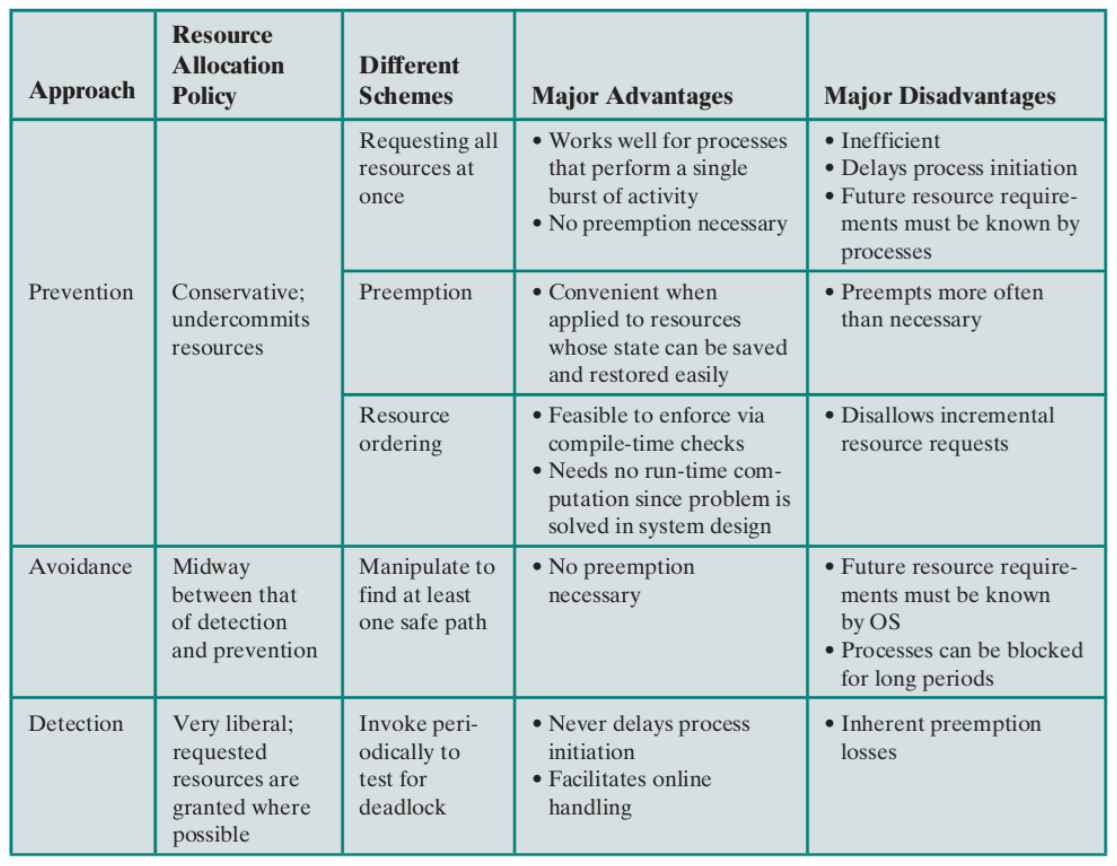
\includegraphics[width=15cm]{unit-15/figures/deadlock-summary.png}
\end{table}
